\documentclass{article}
\usepackage[utf8]{inputenc}
\usepackage[italian]{babel}
\usepackage{amsmath}
\usepackage{amssymb}
\usepackage{siunitx}
\usepackage{tabularray}
\usepackage{graphicx}
\usepackage{float}
\usepackage{minted}
\usepackage[page]{appendix}
\newcommand*{\diam}{\varnothing}
\newcommand*{\best}[1]{{#1}_\text{best}}
\newcommand*{\bestp}[1]{{\left(#1\right)}_\text{best}}
\newcommand*{\pbest}[1]{\left({#1}_\text{best}\right)}
\newcommand*{\pbestp}[1]{\left({\left(#1\right)}_\text{best}\right)}
\newcommand*{\errrel}[1]{\frac{\delta #1}{{#1}_\text{best}}}
\title{
    Laboratorio di Fisica 1\\
    R4: Misura di variabili aleatorie
}
\author{Gruppo 17: Bergamaschi Riccardo, Graiani Elia, Moglia Simone}
\date{8/11/2023 – 15/11/2023}
\makeindex
\begin{document}

\maketitle

\begin{abstract}
    Il gruppo di lavoro ha riprodotto le distribuzioni di Bernoulli e di Poisson attraverso due
    esperimenti distinti, rispettivamente il lancio dei dadi e il decadimento radioattivo.
\end{abstract}

\section{Materiali e strumenti di misura utilizzati}
\begin{center}
    \begin{tblr}{ |Q[l,m]|Q[c,m]|Q[c,m]|Q[c,m]| }
        \hline
        \textbf{Strumento di misura} & \textbf{\:\:\:\:\:Soglia\:\:\:\:\:} & \textbf{Portata} & \textbf{Sensibilità} \\
        \hline
        {Contatore Geiger} & \qty{0}{0} & \qty{0}{0} & \qty{0}{0} \\
        \hline[dashed]
        Metro a nastro & \qty{0.1}{cm} & \qty{300.0}{cm} & \qty{0.1}{cm} \\
        \hline
        \textbf{Altro} & \SetCell[c=3]{l} \textbf{Descrizione/Note} \\
        \hline
        {Sei dadi} & \SetCell[c=3]{l} {
            Usati per riprodurre un processo\\
            bernoulliano.
        } \\
        \hline[dashed]
        {Campione di Torio-232} & \SetCell[c=3]{l} {
            Usato per riprodurre un processo\\
            poissoniano.
        } \\
        \hline
    \end{tblr}
\end{center}

\section{Esperienza e procedimento di misura}
\subsection{Esperienza sulla distribuzione di Bernoulli}
\begin{enumerate}
    \item Eseguiamo 300 lanci simultanei dei sei dadi, riportando in una tabella il risultato di ognuno di essi distinguendoli per il colore;
    \item Acceso e impostato adeguatamente il contatore Geiger (intervalli di tempo di un secondo?), misuriamo per 5? diverse distanze tra contatore e campione il numero di raggi $\gamma$ emessi da quest'ultimo in tot intervalli da un secondo.
\end{enumerate}

Fissato un sistema di riferimento solidale all'apparato di misura, con origine
nella posizione di partenza delle sferette e $\hat{x} = \hat{g}$, possiamo
scrivere la seguente legge del moto:
\[x(t) = \frac{1}{2}g t^2\]
Per ogni sferetta $i$, posto $x\left(\overline{t_i}\right) = d_0 - \frac{1}{2}\diam_i$,
la norma di $\vec{g}$ è ricavabile da:
\[
    g = \frac{2d_0 - \diam_i}{\left(\overline{t_i}\right)^2}
    % \best{g} = \frac{2\best{\left(d_0\right)} - \bestp{\diam_i}}
    %                 {\bestp{\overline{t_i}}^2}
    % \qquad\wedge\qquad
    % \errrel{g} = \frac{2\left(\delta d_0\right) - \delta \diam_i}
    %                   {2\best{\left(d_0\right)} - \bestp{\diam_i}}
    %            + 2\frac{\sigma_{\overline{t_i}}}{\overline{t_i}}
\]
dove determiniamo l'errore su $g$ propagando gli errori su $d_0,\diam_i$ e
$\overline{t_i}$, avendo posto
\[
    \delta\overline{t_i} =
    \sigma_{\overline{t_i}} =
    \frac{\sigma_{t_i}}{\sqrt{100}} =
    \frac{\sigma_{t_i}}{10}.
\]
\\

Di seguito riportiamo gli istogrammi dei tempi e i valori di $g$ così ottenuti.


\begin{figure}[H]
    %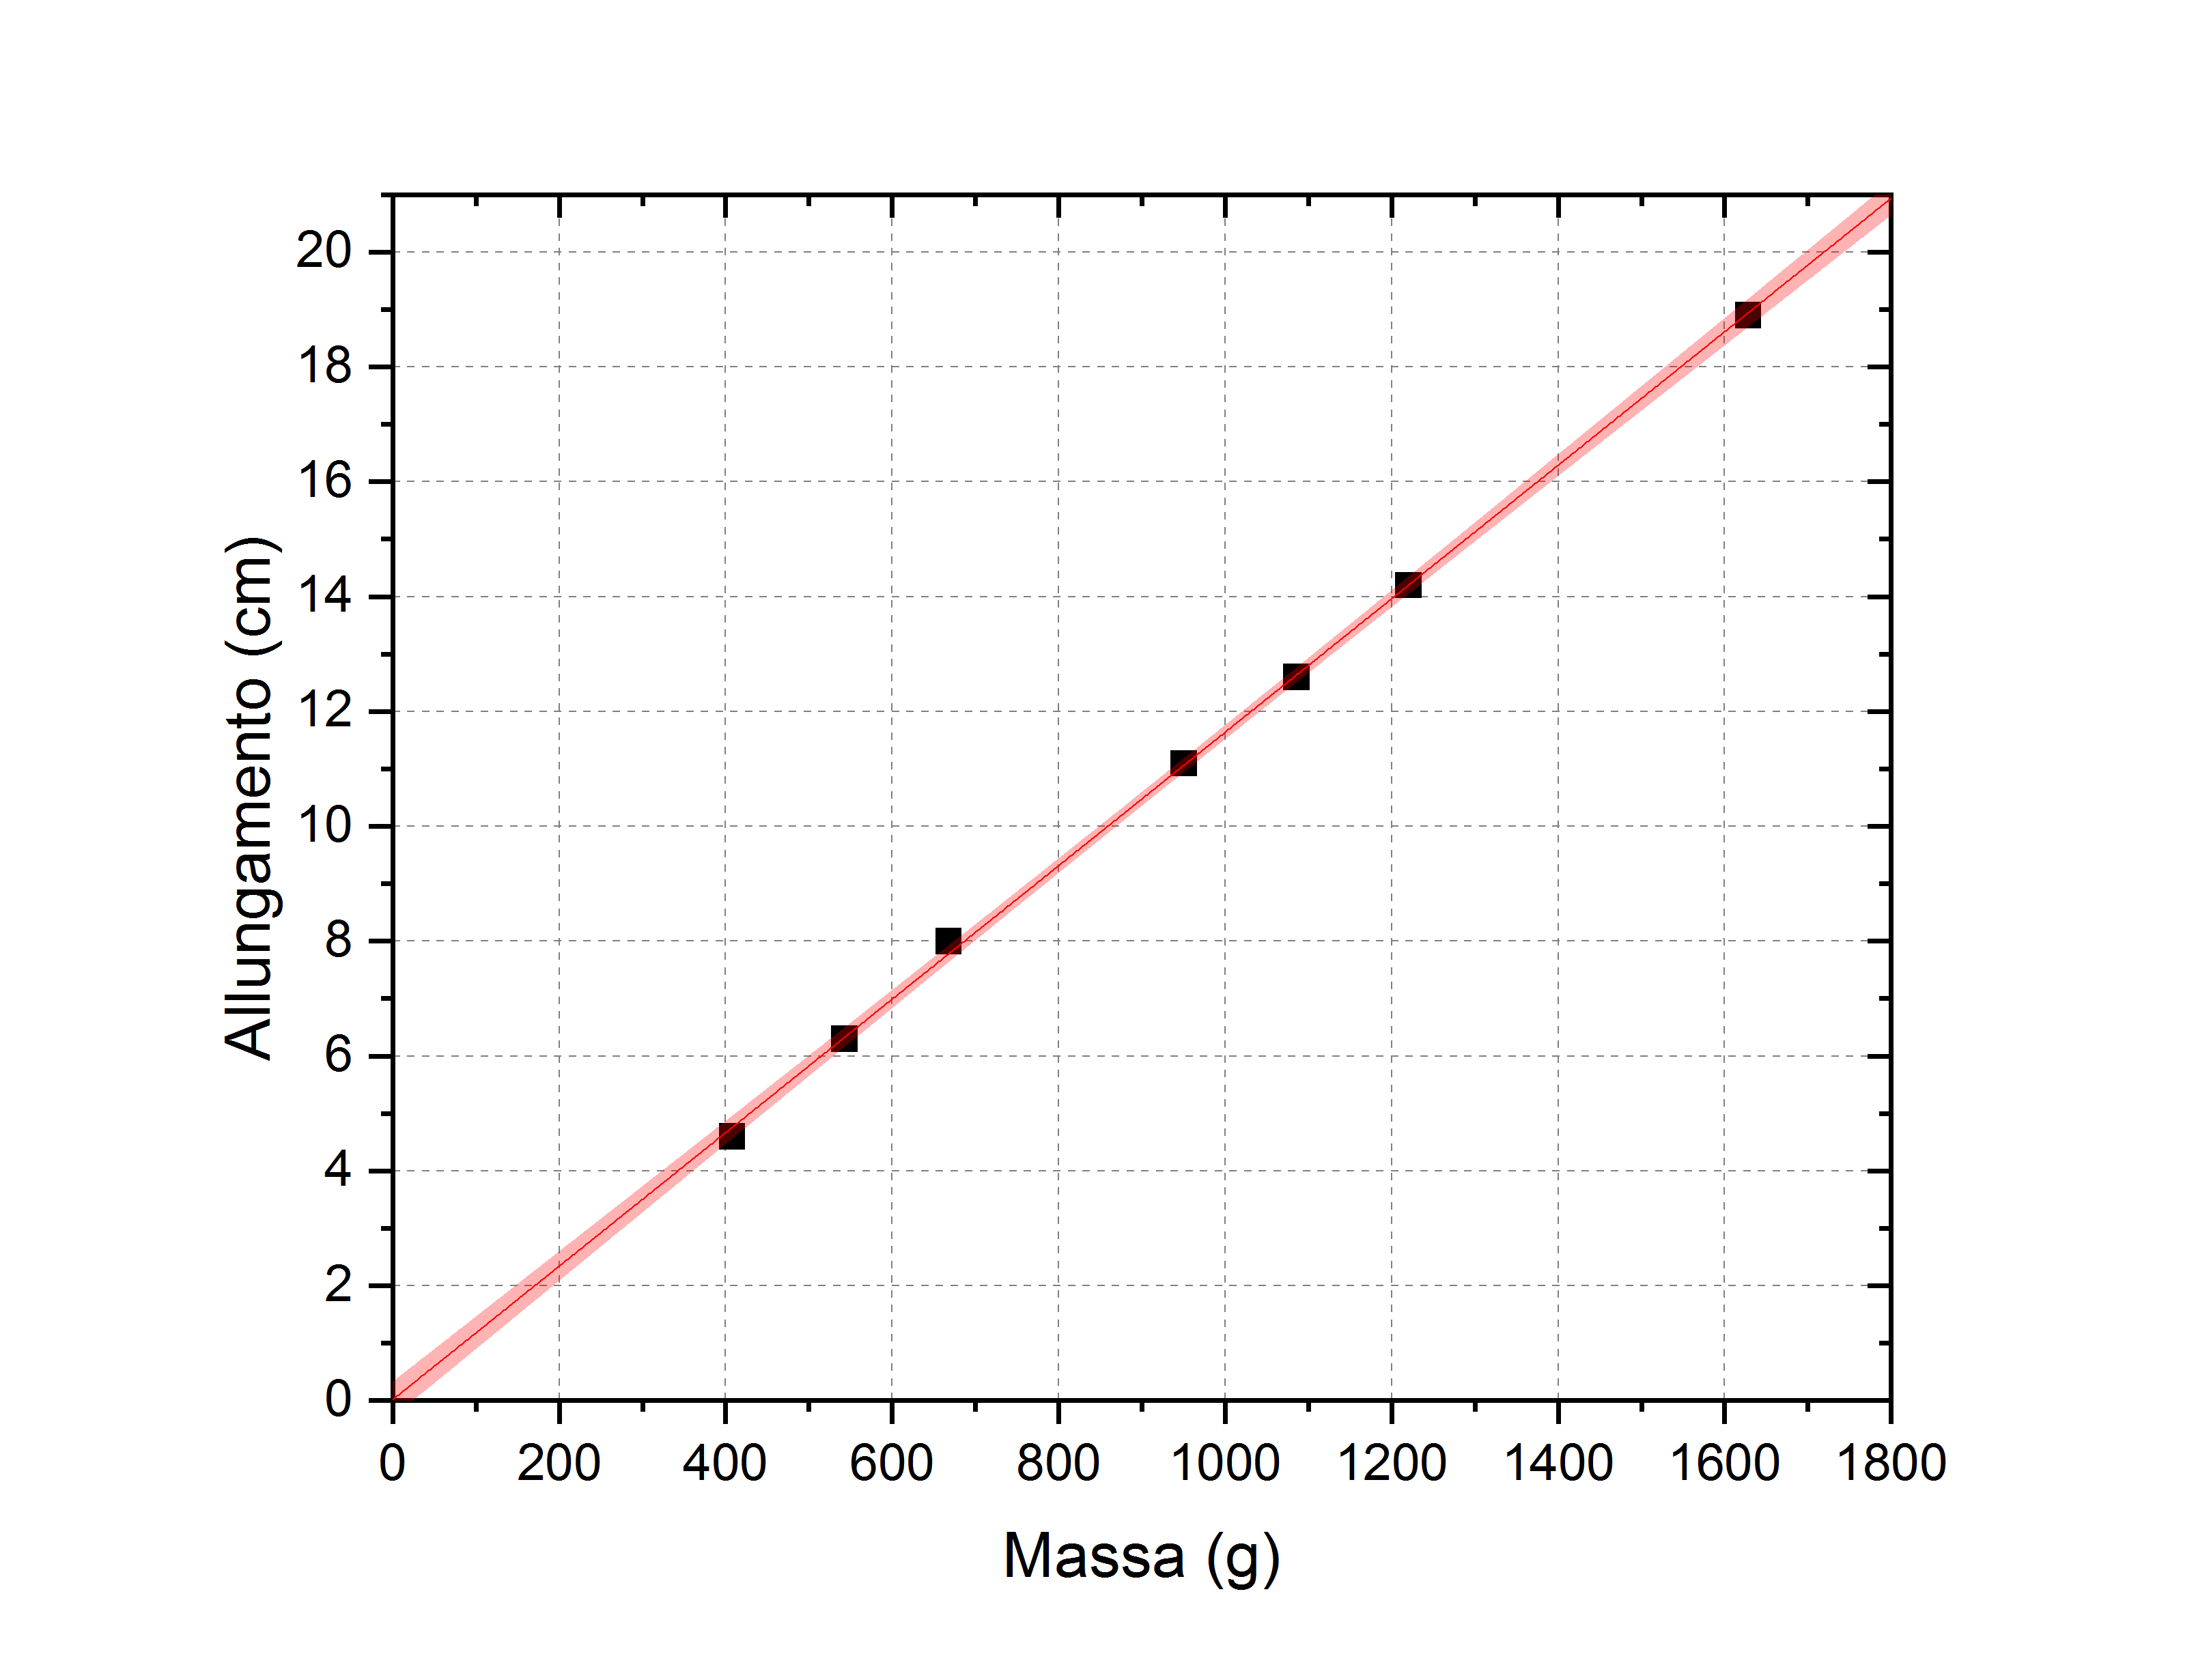
\includegraphics[trim={0 1.8cm 0 0},width=\textwidth]{SaticoReg.jpg}
    \caption{Istogrammi dei dati $t_1$ e $t_2$ raccolti}
\end{figure}
\begin{center}
    \begin{tblr}{ |Q[c,m]|Q[c,m]|Q[c,m]|Q[c,m]|Q[c,m]| }
        \hline
            $i$ &
            $\diam_i\:(\unit{mm})$ &
            $\overline{t_i}\:(\unit{ms})$ &
            $g\:(\unit{m\per s^2})$ &
            $\varepsilon$ \\
        \hline
        A & $24.63\pm0.01$ & $503.62\pm0.03$ & $9.83\pm0.02$ & $1.00$ \\
        \hline[dashed]
        B & $22.23\pm0.01$ & $503.91\pm0.03$ & $9.82\pm0.02$ & $0.93$ \\
        \hline
    \end{tblr}
\end{center}

\subsection{Esperienza sulla distribuzione di Poisson}
\begin{enumerate}
    \item Consideriamo la distanza tra i due fototraguardi e impostiamo i fotodiodi
          del contatore su A+B.
    \item Usando solo
    \begin{enumerate}
        \item Appeso il campione alla molla, allineiamo i due fototraguardi
              aiutandoci con la livella, in modo tale che possano rilevare
              le oscillazioni nel modo più accurato possibile;
        \item Tiriamo leggermente il campione verso il basso e poi lo rilasciamo,
              in modo che il sistema molla inizi a oscillare con direzione
              il più possibile parallela a $\vec{g}$;
        \item Attesa la stabilizzazione dell’oscillazione, avviamo
              l'acquisizione della misura di un tempo (20 periodi)
              $20T_i$.
        \item Ripetiamo molte volte (in tutto $N_{20T_i}$) i punti
              (b) e (c). In particolare, $N_{20T_A} = N_{20T_B} = 25$
              e $N_{20T_C} = N_{20T_{A+B}} = 30$.
    \end{enumerate}
    \item Infine, misuriamo con la bilancia, separatamente,
          la massa della molla $m_m$ e la massa del gancio $m_g$.
\end{enumerate}

Infatti, nel caso dinamico, il contributo di queste masse
\emph{non} si annulla; in particolare, la massa del gancio
contribuisce appieno (in quanto è solidale col grave),
mentre la massa della molla contribuisce per circa
$\frac{1}{3}$. La massa effettiva da considerare per ogni grave
sarà allora:
\[\best{\left(\left(m_\text{eff}\right)_i\right)} = \best{\left(m_i\right)} + \best{\left(m_g\right)} + \frac{1}{3}\best{\left(m_m\right)}\]
\[\delta \left(m_\text{eff}\right)_i = \delta m_i + \delta m_g + \frac{1}{3}\delta m_m\]

Di seguito sono riportate le distribuzioni dei dati raccolti:

\begin{figure}[H]
    %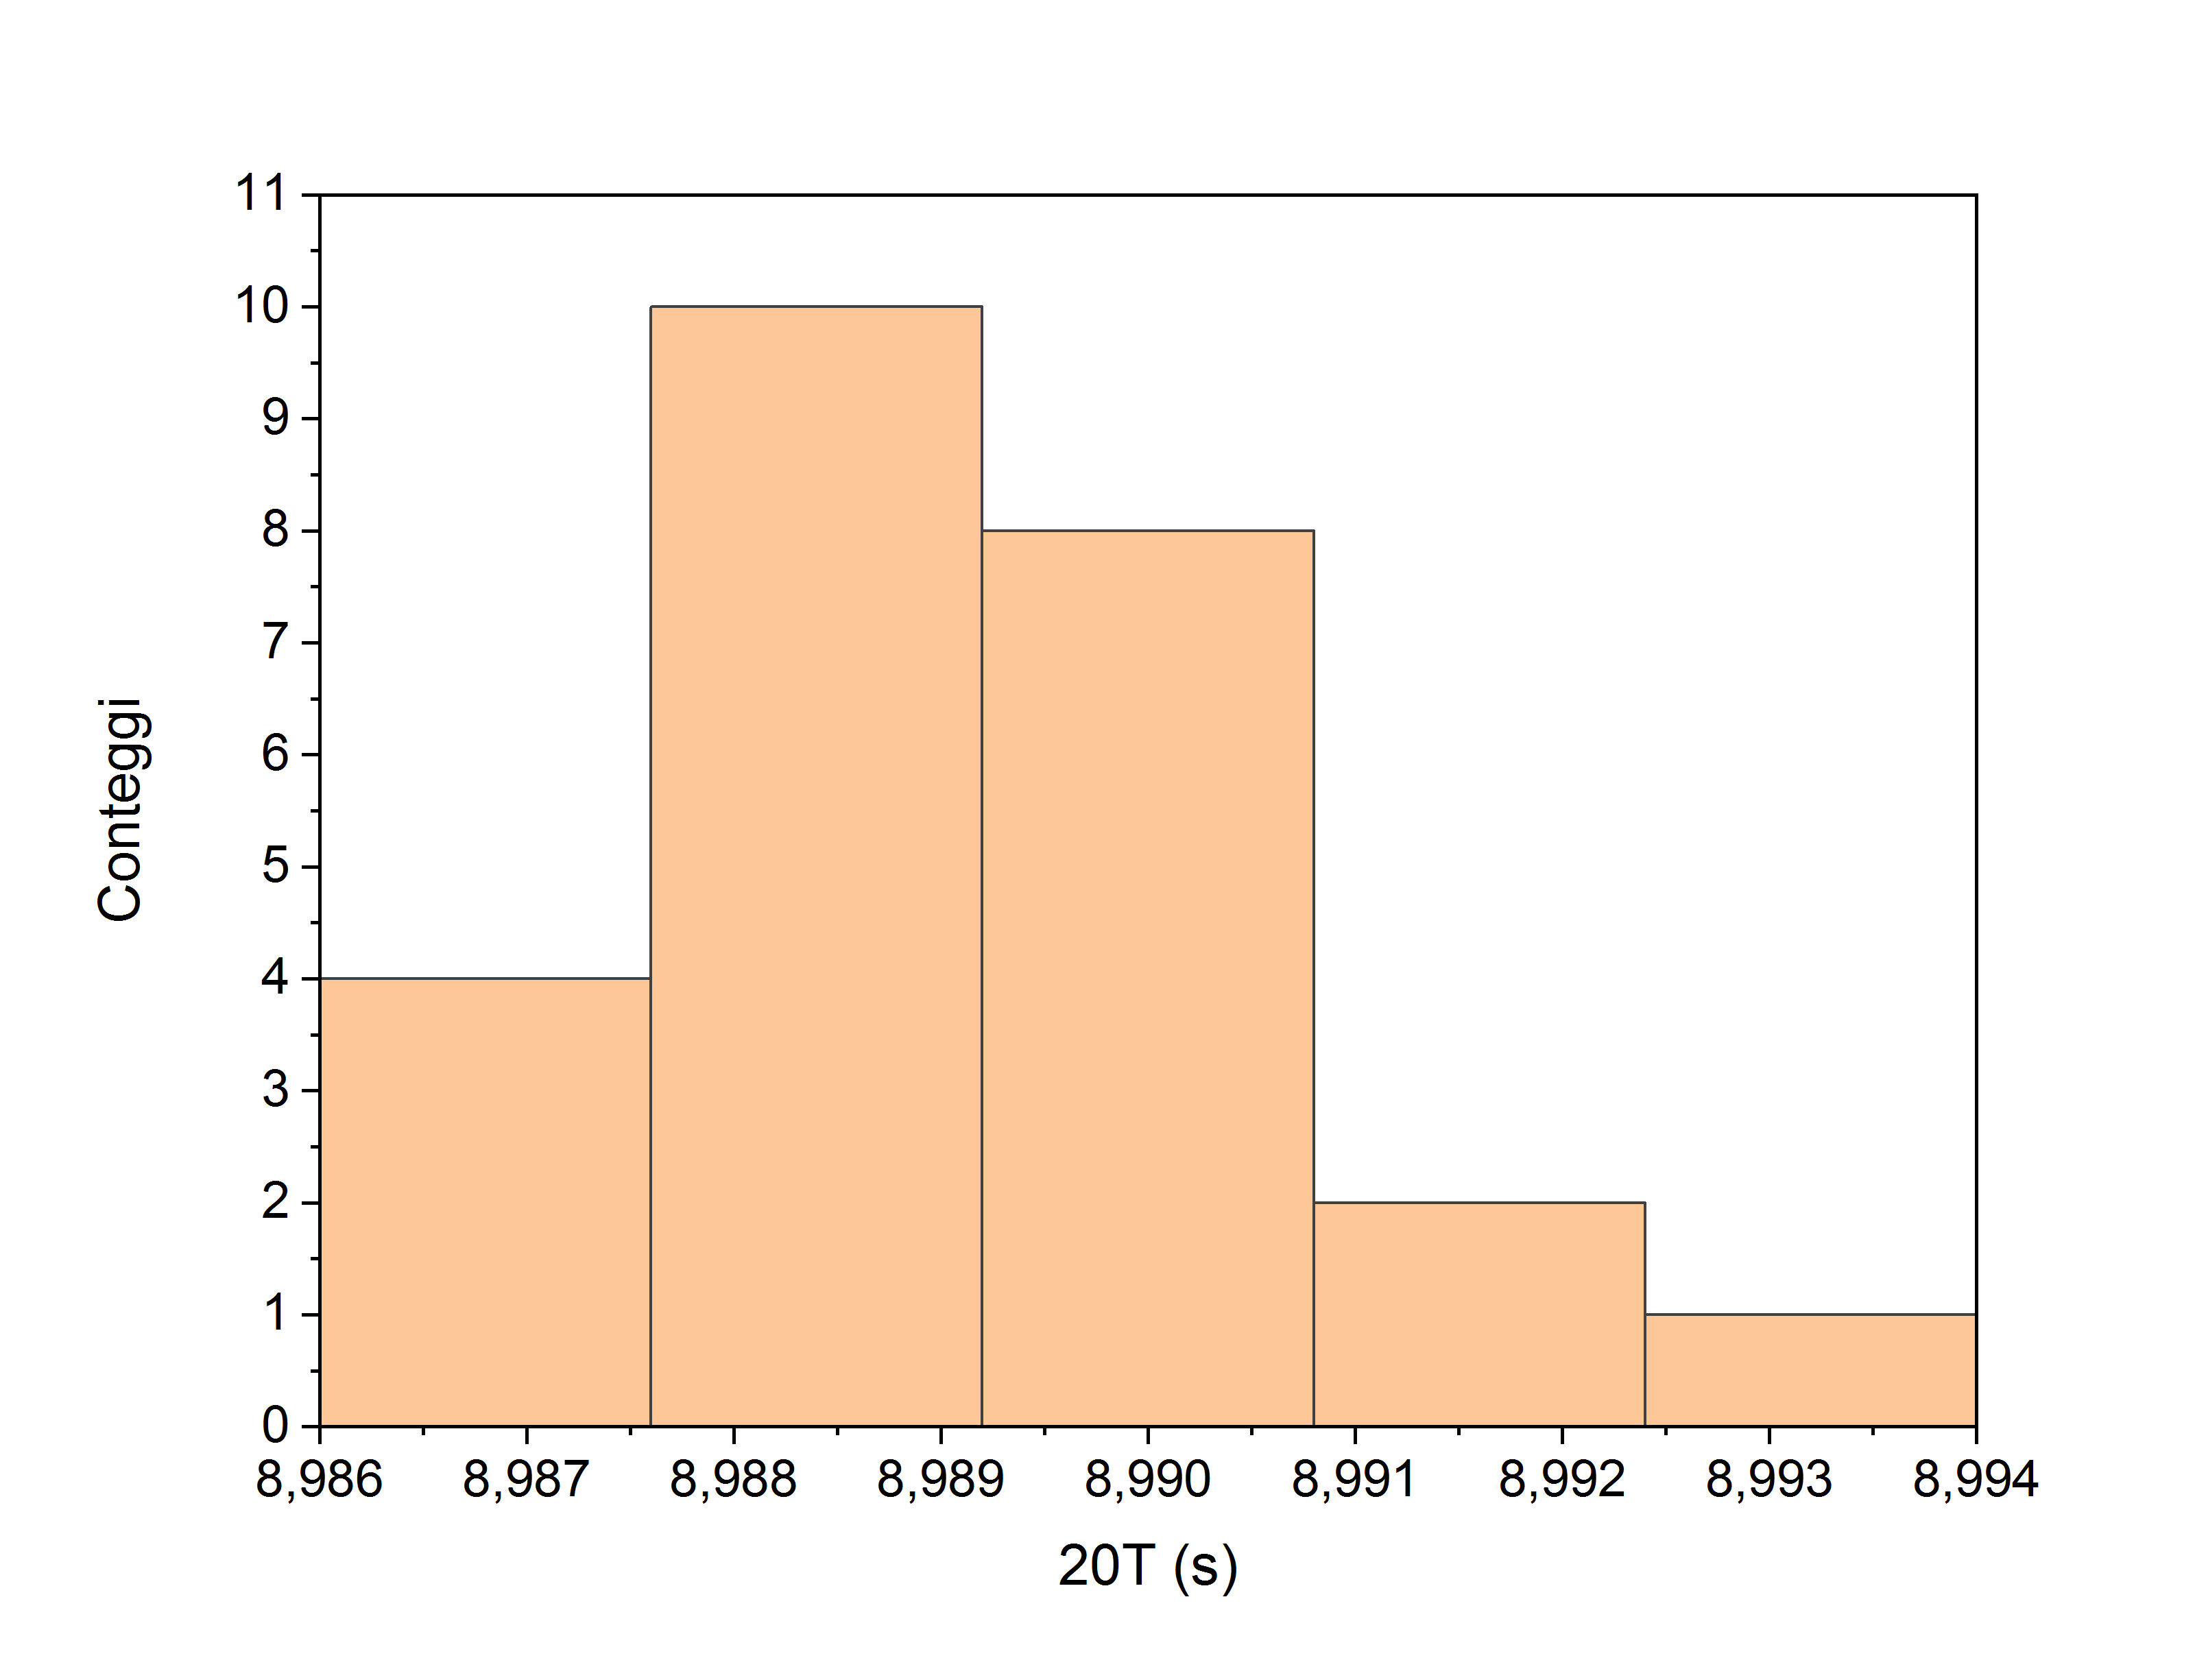
\includegraphics[trim={2cm 1.8cm .7cm 1.5cm},width=.5\textwidth]{Dinamico1.jpg}
    %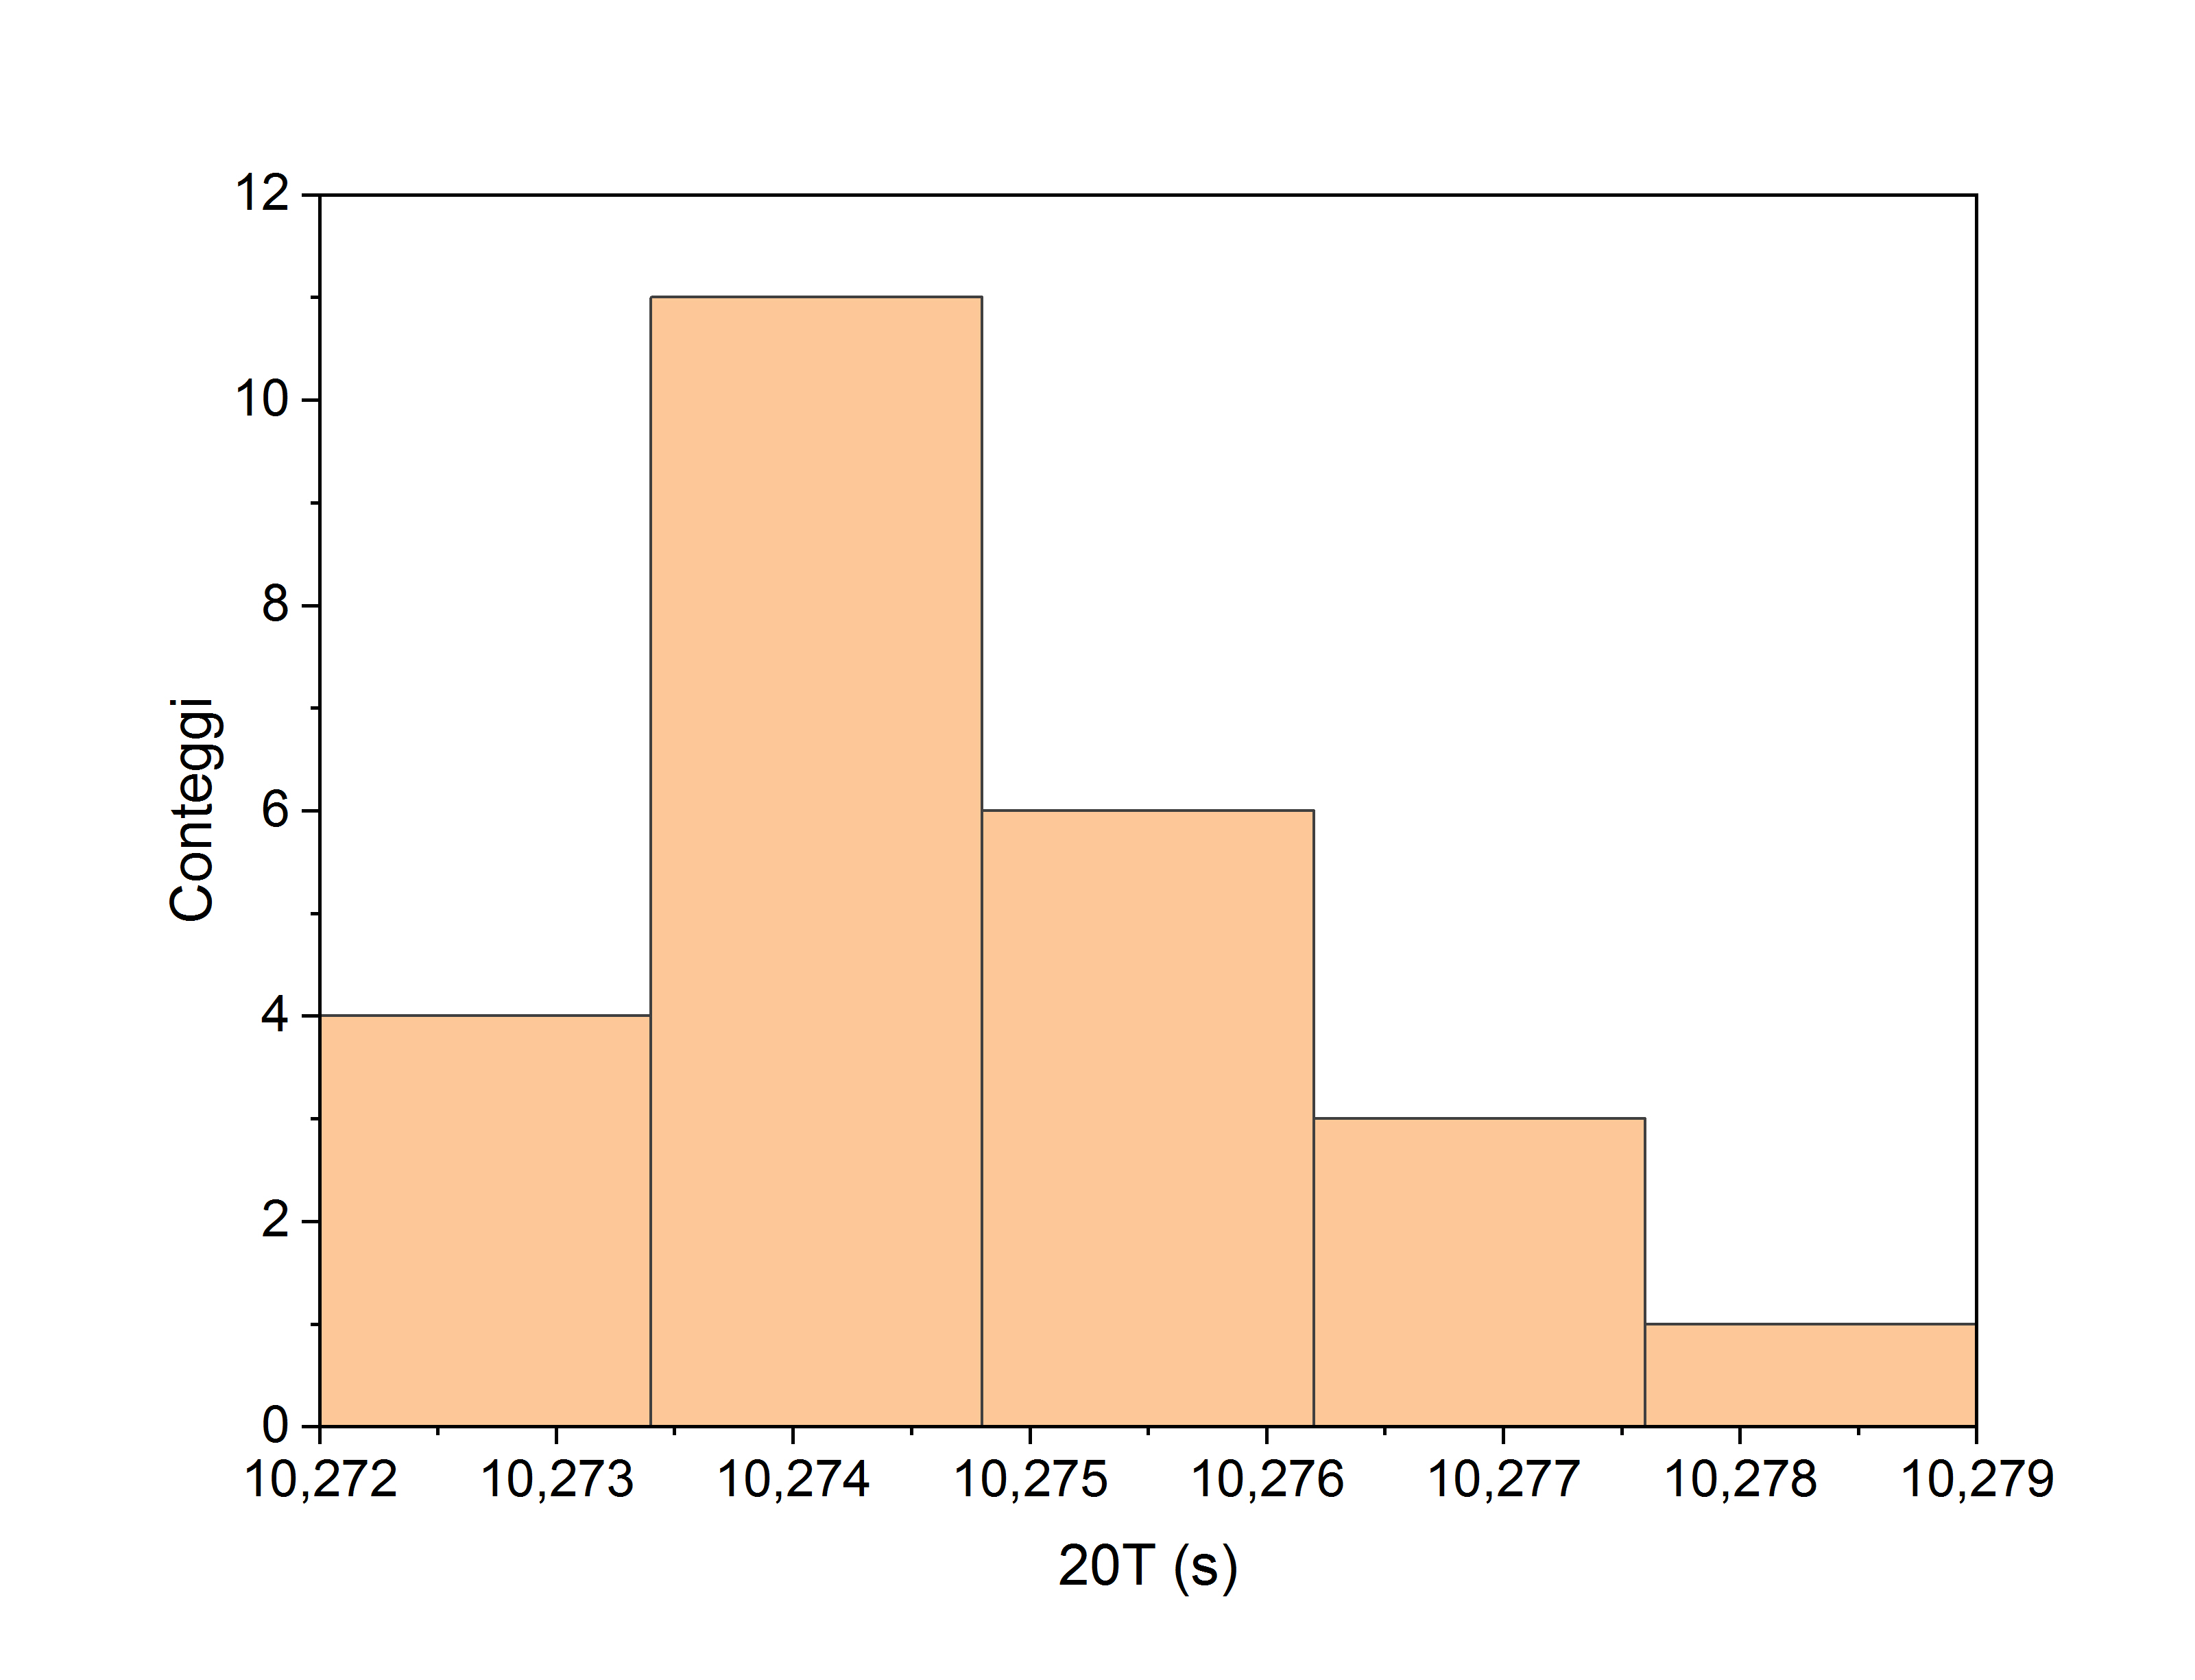
\includegraphics[trim={.7cm 1.8cm 2cm 1.5cm},width=.5\textwidth]{Dinamico2.jpg}
    \caption{Istogrammi dei periodi delle oscillazioni di $A$ e $B$}
\end{figure}\begin{figure}[H]
    %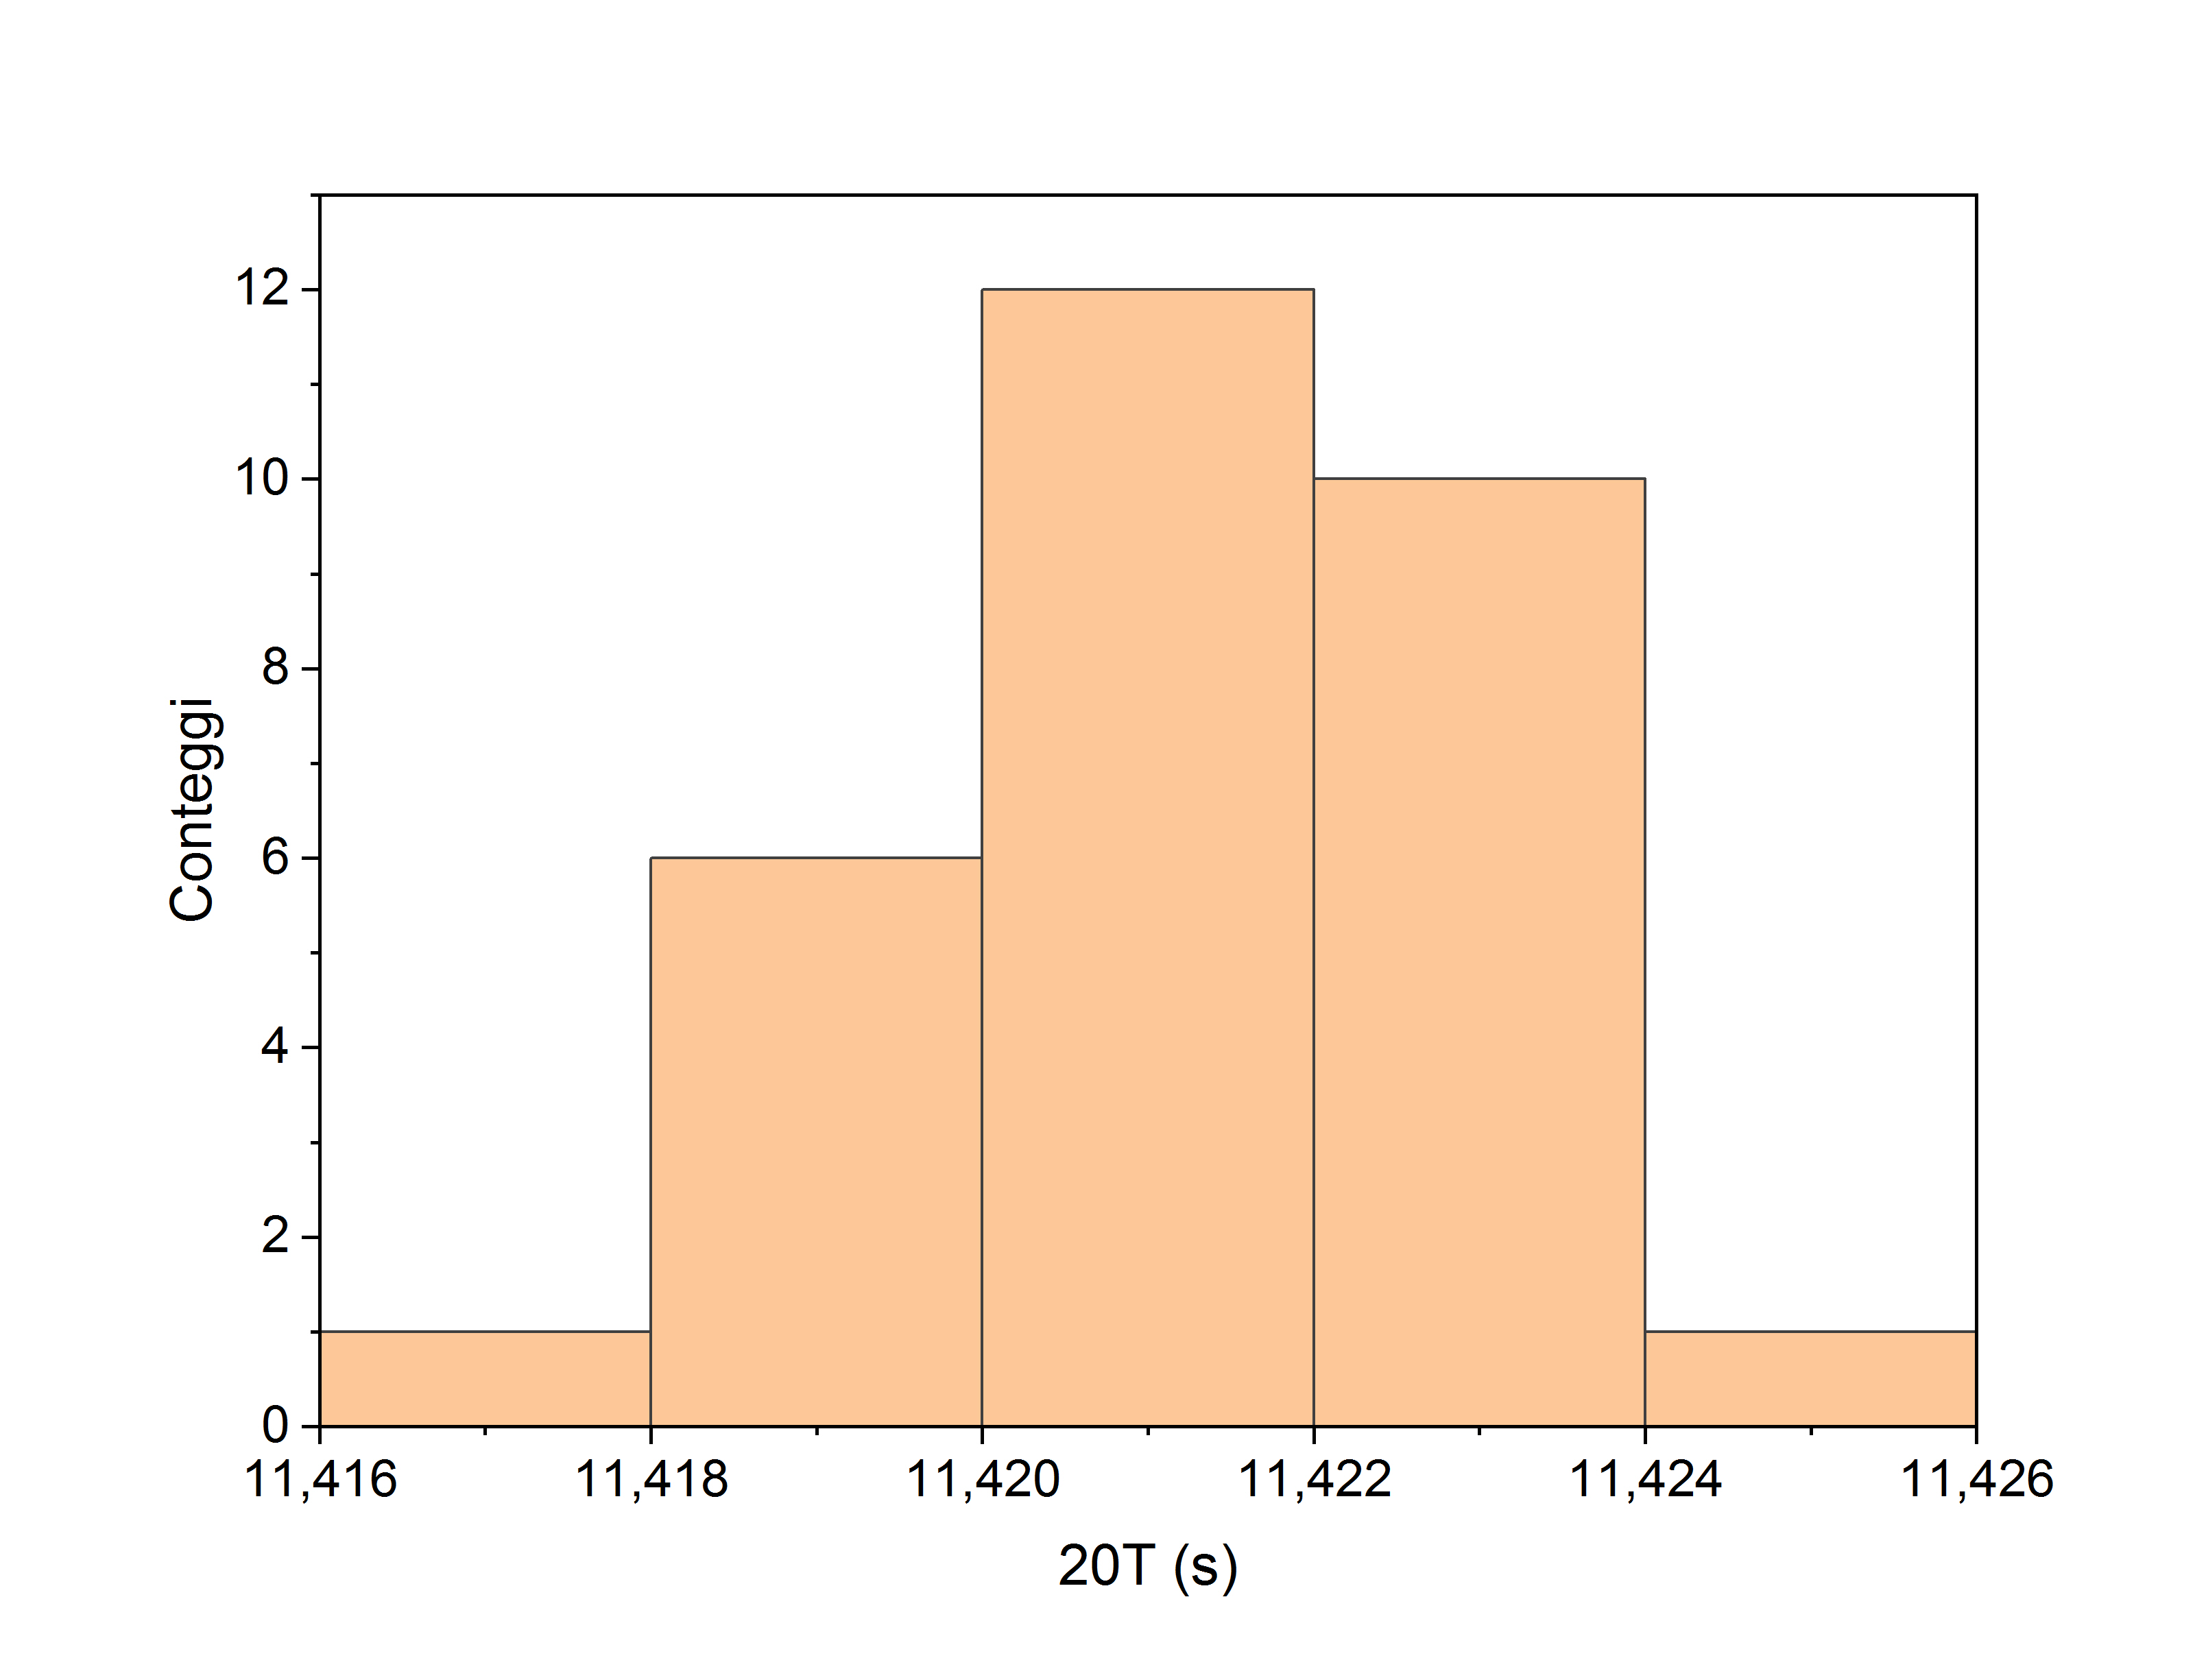
\includegraphics[trim={2cm 1.8cm .7cm 1.5cm},width=.5\textwidth]{Dinamico3.jpg}
    %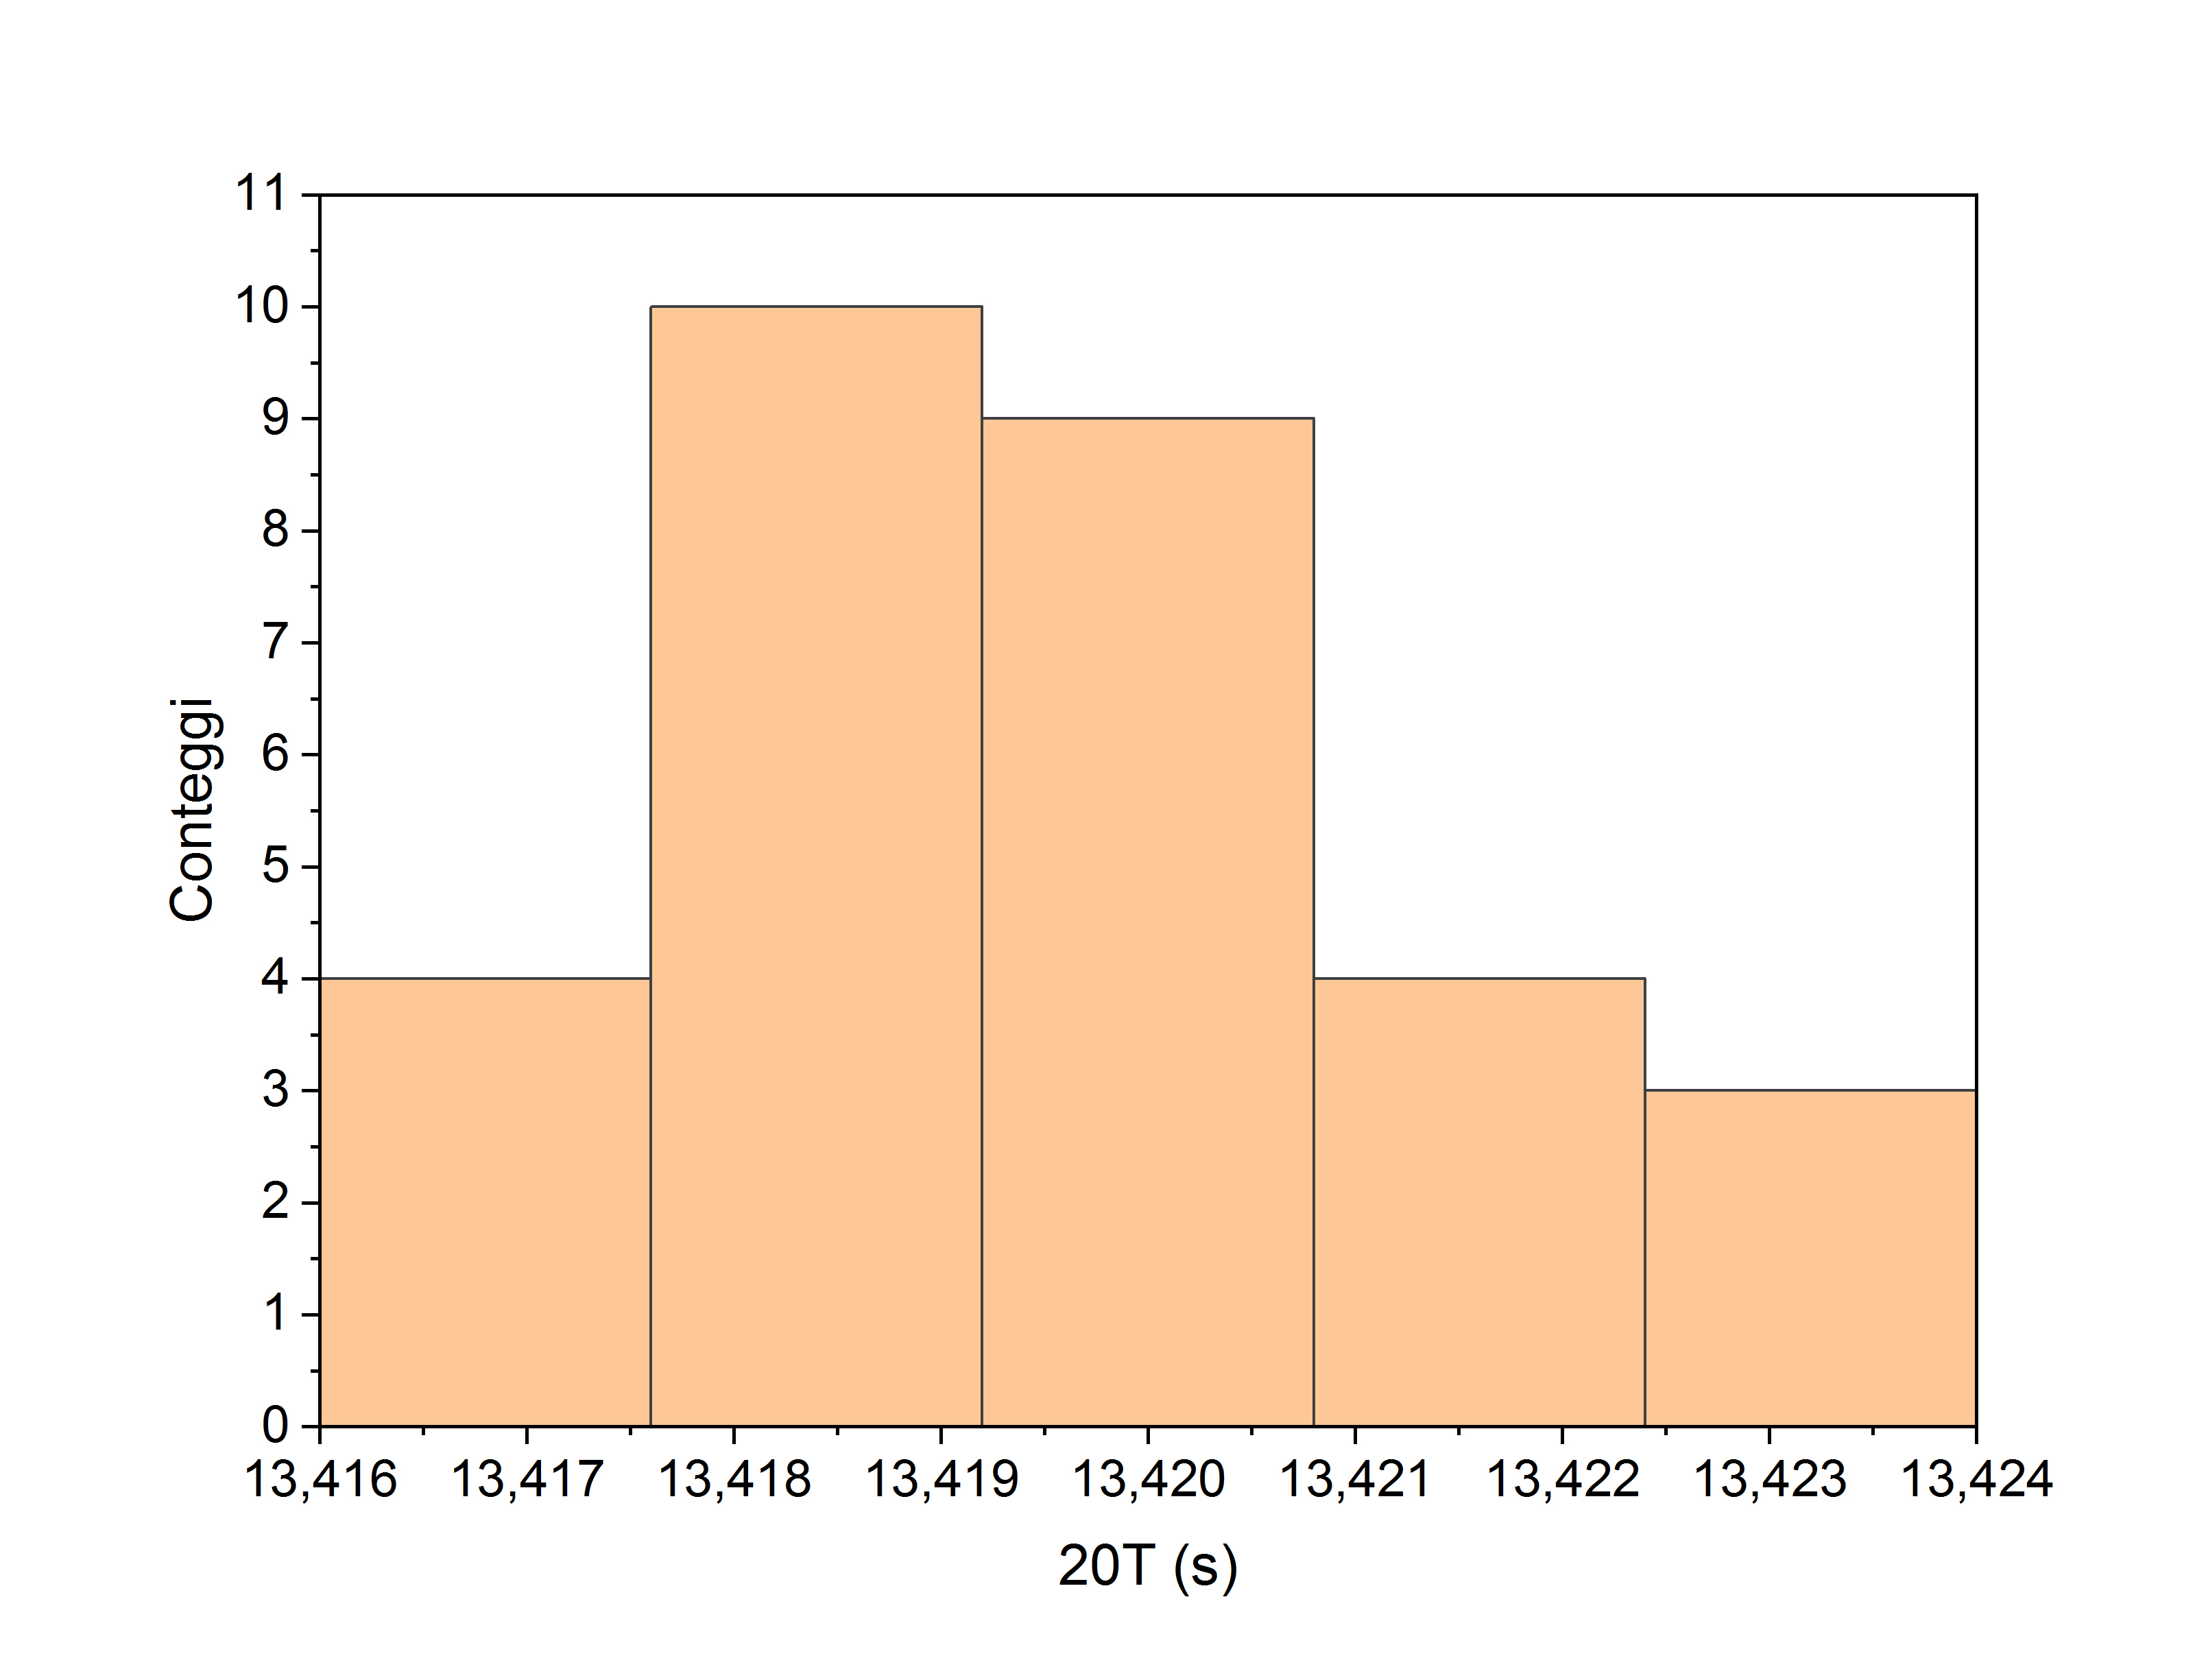
\includegraphics[trim={.7cm 1.8cm 2cm 1.5cm},width=.5\textwidth]{Dinamico4.jpg}
    \caption{Istogrammi dei periodi delle oscillazioni di $C$ e $A+B$}
\end{figure}

Poiché i nostri dati hanno assunto distribuzioni grossolanamente
approssimabili a gaussiane, possiamo procedere al calcolo di $k$,
utilizzando, per ogni grave $i$, i seguenti valori:
\[
    \left(20T_i\right)_\text{best} = \overline{20T_i}
    \qquad\wedge\qquad
    \delta\left(20T_i\right) =
    \sigma_{\overline{20T_i}} =
    \frac{\sigma_{20T_i}}{\sqrt{N_{20T_i}}}
\]
dove $\overline{20T_i}$ e $\sigma_{20T_i}$ indicano rispettivamente
media e deviazione standard dei tempi.

Per determinare la costante elastica della molla, abbiamo effettuato
una regressione lineare (stavolta pesata) sui quadrati dei valori medi
dei tempi ($T_i^2$, con
$\delta T_i^2 = 5 \cdot 10^{-3} (20 T_i)_\text{best} \delta(20 T_i)$
)\footnote[2]{
    La formula per l'errore su $T_i^2$ segue direttamente dalla
    propagazione degli errori:
    \[
        \frac{\delta T_i^2}{\left(T_i^2\right)_\text{best}} = 2\frac{\delta T_i}{{\left(T_i\right)}_\text{best}}
        \qquad
        \delta T_i^2 = 2\left(T_i\right)_\text{best}\delta T_i
        \qquad
        \delta T_i^2 = \frac{\left(20T_i\right)_\text{best}(\delta 20T_i)}{200}
    \]
    da cui quanto riportato sopra.
    Si osservi che $\delta T_i^2$ dipende da
    $\left(20T_i\right)_\text{best}$:
    proprio questo è il motivo dietro alla scelta del metodo pesato
    per la regressione lineare.
} rispetto alla massa $\left(m_\text{eff}\right)_i$, facendo riferimento
alla relazione $T_i^2 = \frac{4\pi^2}{k} \left(m_\text{eff}\right)_i$. Allora, detto $b$ il
coefficiente angolare della retta di regressione, varrà:
\[
    k_\text{best}=\frac{4\pi^2}{b_\text{best}}
    \qquad\wedge\qquad
    \frac{\delta k}{k_\text{best}}=\frac{\delta b}{b_\text{best}}
\]
Si noti che, anche in questo caso, l'intercetta $a$ della retta dev'essere
compatibile con $0$.

Di seguito è riportata la retta di regressione, assieme ai risultati ottenuti:

\begin{figure}[H]
    %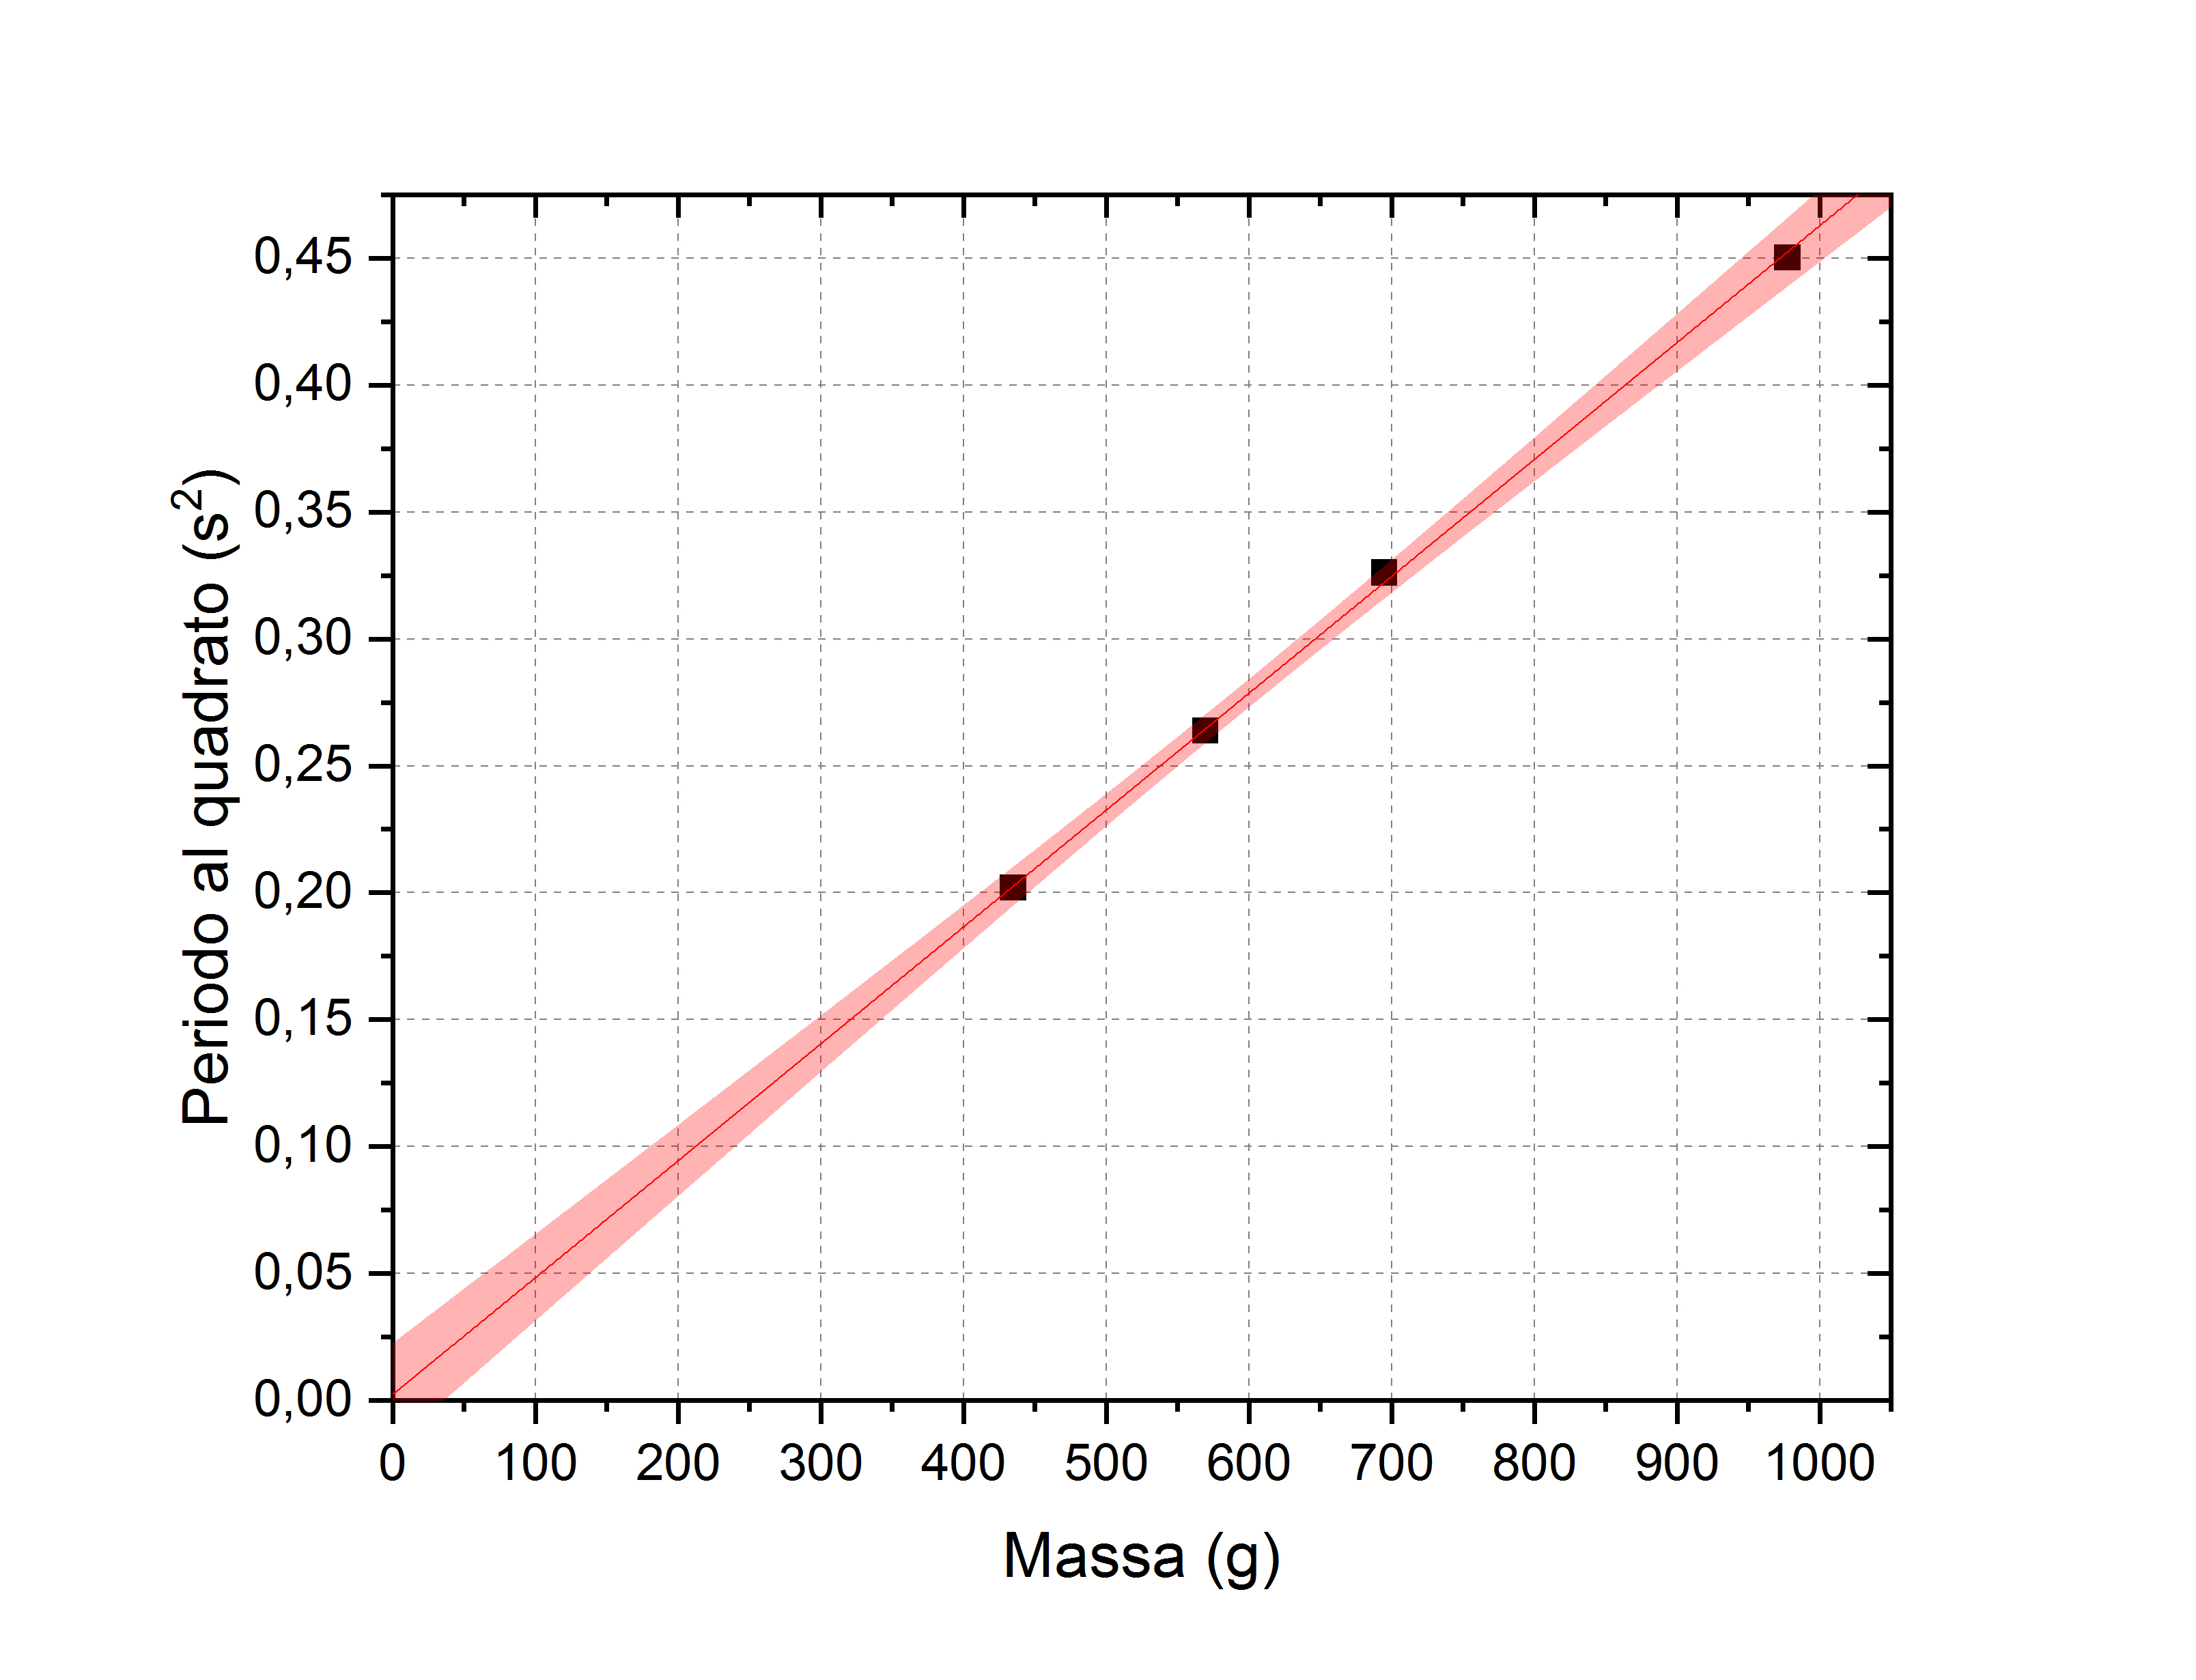
\includegraphics[trim={0 1.8cm 0 0},width=\textwidth]{DinamicoReg.jpg}
    \caption{
        La retta di regressione (in rosso)
        e la sua regione di incertezza (in rosa).
    }
\end{figure}

\begin{itemize}
    \item $a = \left(0.02\pm0.19\right)\unit{cm}$ (compatibile con 0)
    \item $
        b = \left(4.604\pm0.002\right)\cdot10^{-4}\;\unit{s^2\per g}
          = \left(46.04\pm0.02\right)\cdot10^{-2}\;\unit{s^2\per kg}
    $
    \item $k = \left(85.74\pm0.04\right)\unit{N\per m}$
\end{itemize}


\section{Conclusioni}
Per valutare numericamente la consistenza tra i due valori di $k$ ottenuti,
abbiamo calcolato il seguente valore (numero puro):
\[
    \varepsilon =
    \frac{
        \left|\left(k_\text{statica}\right)_\text{best} - \left(k_\text{dinamica}\right)_\text{best}\right|
    }{
        \delta k_\text{statica} + \delta k_\text{dinamica}
    }
\]
Allora $k_\text{statica}$ e $k_\text{dinamica}$ sono consistenti se e solo se $\varepsilon \le 1$.

Nel nostro caso, $\varepsilon = 1.33$. Il gruppo di lavoro ha ipotizzato che
questa inconsistenza (comunque contenuta, seppur non trascurabile) fra le due
misure possa essere ragionevolmente giustificata dalla difficoltà incontrata
nel ridurre al minimo le oscillazioni in direzione perpendicolare a $\vec{g}$;
considerato inoltre che la posizione dei fototraguardi non era ottimale, ciò
potrebbe avere ulteriormente influenzato la distribuzione dei tempi. È in
effetti possibile osservare che le distribuzioni da noi ottenute non sono,
il più delle volte, del tutto simmetriche: la moda sembra essersi spostata
leggermente a sinistra – un possibile sintomo dell'influenza di un
errore sistematico sulle misure.

\begin{appendices}
    \section{Codice Rust per $5\cdot10^{12?}$ lanci di dadi}
    Qui riportiamo il codice Rust, da noi scritto, che ci ha permesso di
    lanciare virtualmente $5\cdot10^{12?}$ dadi in maniera estremamente
    efficiente.

    \inputminted[linenos, mathescape]{rust}{src/main.rs}
\end{appendices}

\end{document}
